\documentclass[12pt]{article}
\usepackage{sbc-template}
\usepackage{graphicx,url}
\usepackage{xspace}
\usepackage[brazil]{babel}
\usepackage[latin1]{inputenc}
\usepackage[T1]{fontenc}
\usepackage{indentfirst}
\usepackage{amsmath}

\newcommand{\AOSD}{Projeto de Sistemas Orientados � Aplica��o}
\newcommand{\epos}{\textsc{Epos}}
\newcommand{\EPOS}{\textsc{Embedded Parallel Operating System}}
\newcommand{\aosd}{\textsc{AOSD}}
\newcommand{\tos}{\textsc{TinyOS}}
\newcommand{\framework}{\textit{framework}}
\newcommand{\ELUS}{\textsc{Elus}}
\newcommand{\elus}{\textsc{Epos Live Update System}}

\newcommand{\X}{$\bullet$}

\newcommand{\en}[1]{\emph{#1}}
\newcommand{\class}[1]{{\sffamily\bfseries{#1}}}
\newcommand{\componente}[1]{\texttt{#1}}
\newcommand{\method}[1]{\componente{#1}}
\newcommand{\proxy}{\componente{Proxy}}
\newcommand{\agent}{\componente{Agent}}
\newcommand{\handle}{\componente{Handle}}
\newcommand{\stub}{\componente{Stub}}
\newcommand{\adapter}{\componente{Adapter}}
\newcommand{\scenario}{\componente{Scenario}}
\newcommand{\msg}{\componente{Message}}
\newcommand{\vtable}{\componente{vtable}}
\newcommand{\etp}{\textsc{Elus Transport Protocol}}
\newcommand{\ETP}{\textsc{Etp}}
\newcommand{\rt}{\componente{Reconfigurator}}

\newcommand{\fig}[4][thb]{
  \begin{figure}[#1] {\centering{\includegraphics[#4]{fig/#2}}\par}
    \caption{#3\label{fig:#2}}
  \end{figure}
}

\usepackage{listings}
\lstset{keywordstyle=\bfseries, flexiblecolumns=true}
\lstloadlanguages{[ANSI]C++,HTML}
\lstdefinestyle{prg} {basicstyle=\footnotesize, lineskip=-0.2ex, showspaces=false,breaklines=true,showstringspaces=false,numbers=left,numbersep=-5pt,frame=single,stepnumber=1}

\newcommand{\prg}[3][tbp]{
  \begin{figure}[#1]
      \lstinputlisting[language=C++,style=prg]{fig/#2.cc}
    \caption{#3\label{prg:#2}}
  \end{figure}
}

\sloppy

%\title{Dissemina��o de Dados para Reprograma��o de Software em SOs Embarcados}
\title{Uma Estrutura de Reprograma��o em Rede para Sistemas Operacionais Embarcados}

%Qual nome vai primeiro???
\author{Rodrigo Steiner, Giovani Gracioli e Ant�nio Augusto Fr�hlich}

\address{Laborat�rio de Integra��o Software e Hardware (LISHA)\\
  Universidade Federal de Santa Catarina (UFSC)\\
  Caixa Postal 476, 88049-900, Florian�polis, SC, Brasil
  \email{\{rodrigo,giovani,guto\}@lisha.ufsc.br}
}

\begin{document}

\maketitle

\begin{resumo}
Este artigo apresenta uma estrutura de reprograma��o de software em rede para sistemas embarcados. Tal estrutura foi desenvolvida no sistema operacional EPOS e � formada por um protocolo de dissemina��o de dados e um ambiente de suporte de sistema operacional que isola os componentes do sistema em unidades f�sicas independentes de posi��o de mem�ria, permitindo que sejam atualizados em tempo de execu��o. A estrutura foi testada em nodos reais e avaliada em termos de consumo de mem�ria, tempo de dissemina��o e de reprograma��o.

\end{resumo}

\begin{abstract}
This paper presents a software network reprogramming structure for embedded systems. Such a structure was developed in the EPOS operating systems and it is composed by a data dissemination protocol and an operating system support environment that isolates the system components in memory position independent physical units, allowing their updating at execution time. The structure was tested in real nodes and evaluated in terms of memory consumption, dissemination and reprogramming time.
\end{abstract}

\section{Introduction}
% Reprogramao, estrutura + protocolo
% O que  um protocolo de disseminao
% Importncia de um prot. de diss.
% Importncia de uma boa estrutura
% Ex. de uso: reprogramao RSSF
% Contribuio: infra-estrutura p/ disseminao e reprogramao
% Organizao do artigo

%Reprogramming the software of a program in execution is a feature present in most computer environments.
%A wide range of applications make use of some reprogramming method: from internet browsers to dedicated systems, as controllers in vehicles for instance.
%Due to the limited resources of embedded systems, the software reprogramming infrastructure is different from that implemented in conventional computer environments.
%Moreover, some of these dedicated systems, as Wireless Sensor Networks (WSNs), are formed by a big amount of nodes, in which collecting and reprogramming all nodes is impractical. 

%Wireless Sensor Networks (WSN), are typically formed by a big amount of nodes, in which collecting and reprogramming all nodes is impractical.
A software reprogramming infrastructure for a Wireless Sensor Network (WSN) is composed of a data dissemination protocol and a structure capable of organizing the data in the system's memory. By using an embedded Operating System (OS) it is possible to provide for embedded applications an infrastructure to hide this data organization. Usually, the reprogramming structures present in OSs are composed of updatable modules. These modules are memory position independent and are replaced at runtime~\cite{sos}~\cite{contiki}. 

In addition, it is essential that all new data of one or more modules is correctly received by all nodes involved in the reprogramming process. In order to provide safe data transfer, a data dissemination protocol is used together with the OS infrastructure.
%In general, a dissemination protocol works as follows: the dissemination begins from a base station responsible to transfer the new data to its neighbor nodes. Once a node receives the new data, it is capable of retransmitting it to its own neighbors.  The process repeats until the entire network is up to date~\cite{moap}~\cite{deluge}.
%Thus, if a node A is neighbor of a node B, and the node B has A and C as neighbors, the node B after receiving the new data from the node A will retransmit it to the node C. The process repeats for all nodes until the entire network is up to date~\cite{moap, deluge}.

Epos Live Update System (\ELUS{}) is an OS infrastructure for software updating that has better performance in terms of memory consumption, method invocation time, and reconfiguration time when compared to related works~\cite{Gracioli:2010}.
%Although this favorable result, we identifed that memory consumption of \ELUS{} could be improved.
Although this favorable result, \ELUS{} memory consumption could still be improved.
Furthermore, \ELUS{} does not have any support for data dissemination. 

%In summary, in this paper, we make the following contributions:
%\begin{itemize}
%	\item We improved the memory consumption of \ELUS{} by using C++ templates specialization techniques (more than 50\% of improvement). %\ELUS{} is implemented around the EPOS metaprogrammed framework~\cite{Frohlich:2001}. Thus, some code regions are duplicated due to the use of templates. We identified some of these regions and applied a template specialization technique~\cite{stroustrup:2000}.
%	\item We provide a domain engineering analysis considering the data dissemination protocols characteristics. The protocols characteristics are decomposed into a feature diagram that shows common and variable features present in different protocols.
%	\item We integrate a data dissemination protocol to \ELUS{} and evaluate the new infrastructure in terms of memory consumption and dissemination and reprogramming times. %As result, we provide a lightweight software reprogramming infrastructure for resource-constrained embedded systems.
%\end{itemize}

%In this paper we make the following contributions: (i) we have improved the memory consumption of \ELUS{} by using C++ templates specialization techniques; (ii) we provide a data dissemination protocol domain engineering analysis considering protocols characteristics, and integrate our developed protocol to \ELUS{}; and (iii) we evaluate the new infrastructure in terms of memory consumption, and dissemination and reprogramming times.
In this paper we make the following contributions: (i) we develop and integrate a data dissemination protocol to \ELUS{}; (ii) we improve the memory consumption of \ELUS{} by using C++ templates specialization techniques; and (iii) we evaluate the new infrastructure in terms of memory consumption, and dissemination and reprogramming times.

%The rest of this paper is organized as follows.
%Section~2 presents the related work.
%Section~\ref{sec:ddp} shows the designed dissemination protocol and compares its characteristics to other proposed protocols.
Section~\ref{sec:ddp} presents the design of the developed dissemination protocol.
Section~\ref{sec:integration} presents the integration between the dissemination protocol and \ELUS{}.
The evaluation of the infrastructure is carried out in Section~\ref{sec:evaluation}.
Finally, Section~\ref{sec:conc} concludes the paper.


\section{Trabalhos Relacionados}
% Protocolos de Dissemina��o
% - tabela comparativa
% SOs embarcados
% - tinyos, sos, mantisos, retos, nano-kernel

\subsection{Protocolos de Dissemina��o}
%MOAP
\textit{Multi-hop Over the Air Programming} � um mecanismo de distribui��o de c�digo projetado priorizando o consumo de energia e mem�ria em detrimento da lat�ncia \cite{moap}. O \textsc{MOAP} utiliza um mecanismo de dissemina��o chamado \textit{Ripple}, que distribui os dados de vizinhan�a em vizinhan�a. Em cada vizinhan�a apenas um pequeno subconjunto de nodos (de prefer�ncia apenas um) funcionam como emissores, enquanto os restantes s�o receptores. Quando os nodos recebem todos os dados eles podem se tornar emissores para seus pr�prios vizinhos (que estavam fora do alcance do emissor original). Para evitar que nodos se tornem emissores em uma vizinhan�a que j� possua um, o mecanismo utiliza uma interface divulga/inscreve, nodos emissores divulgam sua vers�o e todos os interessados se inscrevem. Caso um emissor n�o receba inscri��es ele fica em sil�ncio.

%Deluge
\textit{Deluge} � um protocolo de dissemina��o projetado para propagar uma grande quantidade de dados de forma r�pida e confi�vel. Ele compartilha v�rias ideias com o \textsc{MOAP}, como o uso de NACKs, pedidos de retransmiss�o \textit{unicast} e transmiss�o de dados \textit{broadcast} \cite{deluge}. Com o intuito de limitar a quantidade de informa��es que um receptor deve manter, possibilitar atualiza��es incrementais e permitir que os nodos continuem a dissemina��o antes de possu�rem todos os dados, o protocolo utiliza o conceito de p�ginas. Os dados s�o divididos em \emph{P} p�ginas, sendo que uma p�gina nada mais � do que um conjunto de \emph{N} pacotes. Utilizando um vetor de idades para descrever a idade de cada p�gina, os nodos s�o capazes de determinar quando uma p�gina mudou e se necessitam ou n�o requisit�-la. Exigindo que os nodos recebam uma p�gina por vez, pode-se utilizar um mapa de bits de apenas \emph{N} bits para gerenciamento de segmentos, pois n�o � mais necess�rio manter registros de todos os pacotes ao mesmo tempo.

%MNP
\textit{Multi-hop Network Programming} (MNP) � um protocolo de reprograma��o em rede cujas principais caracter�sticas incluem um mecanismo para sele��o de emissor e uma abordagem para reduzir o uso da mem�ria RAM \cite{mnp}. Assim como no \textsc{MOAP} a dissemina��o ocorre de vizinhan�a em vizinhan�a e um nodo s� pode se tornar emissor ap�s receber todos os dados. Atrav�s do algoritmo para sele��o de emissor, um nodo decide se deve transmitir o c�digo ou n�o. O objetivo deste algoritmo � o de garantir que a qualquer momento apenas um nodo esteja transmitindo os dados por vez, e que este transmissor seja o que vai causar maior impacto, em outras palavras, o que tiver um maior n�mero de receptores. � importante ressaltar que o algoritmo n�o garante encontrar o emissor ideal, todavia, ele seleciona ``bons'' emissores e reduz o n�mero de colis�es.

%Infuse
\textit{Infuse} � um protocolo de dissemina��o de dados baseado em uma comunica��o sem colis�es devido ao uso do MAC (\textit{Medium Access Control}) TDMA (\textit{Time Division Multiple Access}) \cite{infuse}. Este protocolo requer que os nodos conhe�am tanto a sua localiza��o como a de seus vizinhos, classificando-os em predecessores e sucessores. Assim um nodo ouve durante a faixa de tempo de seus predecessores para receber os dados e transmite durante a sua. A Tabela \ref{tab:prot} apresenta as prioridades dos protocolos analisados.

%Sprinkler
%\textit{Sprinkler} � um servi�o de dissemina��o de dados projetado para ser energ�ticamente eficiente atrav�s da computa��o de um subconjunto de nodos emissores e do uso de TDMA \cite{sprinkler}. Assim como o \textit{Infuse}, o \textit{Sprinkler} tamb�m requer que os nodos saibam a sua localiza��o. Al�m disto, este mecanismo assume que a distribui��o dos nodos possua uma densidade m�nima. Partindo destas duas premissas um CDS (\textit{Connected Dominating Set}) � computado e sobre este conjunto s�o calculadas faixas de tempo para uma transmiss�o TDMA atrav�s do algoritmo de colora��o D-2. A dissemina��o � dividida em duas fases: \textit{Streaming}, onde apenas os nodos pertencentes ao CDS transmitem pacotes e \textit{Recovering}, quando nodos n�o pertencentes ao CDS enviam requisi��es por pacotes perdidos.

\subsection{Sistemas Operacionais Embarcados}
Alguns SOs embarcados s�o projetados com uma abstra��o para atualiza��o de software. Atrav�s desta abstra��o � poss�vel realizar reprograma��es em tempo de execu��o sem a necessidade de reiniciar o sistema, desta forma, evitando perda de dados.

%TinyOS
\textsc{TinyOS} � um sistema operacional constitu�do de componentes reutiliz�veis que s�o usados em conjunto formando uma aplica��o espec�fica \cite{tinyos}. Este SO suporta uma ampla gama de plataformas de hardware e tem sido utilizado em v�rias gera��es de nodos sensores, podendo ser considerado o SO mais usado na �rea de RSSF. Ele apresenta um modelo de concorr�ncia orientado a eventos e originalmente n�o suporta reconfigura��o de software. Contudo, todos os protocolos apresentados anteriormente foram implementados utilizando o \textsc{TinyOS}, desta forma possibilitando a reconfigura��o. 
%\textsc{TinyOS} � considerado o SO mais popular para RSSF. � um SO orientado a eventos e originalmente n�o suporta reconfigura��o de software~\cite{hill00system}. Entretanto, diversos trabalhos t�m sido realizados com o intuito de suportar reconfigura��o no \textsc{TinyOS}~\cite{deluge, flexcup, mate}. \textsc{MantisOS} � outro SO para RSSF muito conhecimento no ambiente acad�mico, mas n�o suporta reconfigura��o~\cite{mantis}.

%SOS
\textsc{SOS} � um sistema operacional constitu�do por m�dulos dinamicamente carreg�veis e um \textit{kernel} \cite{sos}. Esses m�dulos enviam mensagens e se comunicam com o \textit{kernel} atrav�s de uma tabela do sistema que cont�m \textit{jumps} relativos. Desta forma o c�digo em cada m�dulo torna-se independente de posi��o da mem�ria, possibilitando altera��es no software de maneira mais eficiente.
%\textsc{SOS} � um SO para RSSF que permite RDS~\cite{sos}. O SO � constru�do em m�dulos que s�o inseridos, removidos ou substitu�dos em tempo de execu��o. Atrav�s do uso de chamadas relativas, o c�digo em cada m�dulo torna-se independente de posi��o da mem�ria. \ELUS{} � conceitualmente similar aos trabalhos relacionados apresentados, por�m a infra-estrutura do framework possui a vantagem de eliminar parte do sobrecusto associado �s tabelas de indire��o com o uso da metaprograma��o est�tica. Tabela~\ref{tab:reconf2} revisa o processo de reconfigura��o nos SOs embarcados analisados.

%Contiki
\textsc{Contiki} � um SO que possui uma estrutura de reconfigura��o semelhante a do \textsc{SOS}. Ele implementa processos especiais, chamados \emph{servi�os}, respons�veis por prover funcionalidades a outros processos~\cite{dunkels04contiki}. Esses servi�os podem ser substitu�dos em tempo de execu��o atrav�s de uma \emph{interface stub} respons�vel por redirecionar as chamadas das fun��es para uma \emph{interface de servi�o}, que possui ponteiros para as implementa��es atuais das fun��es do servi�o correspondente. A Tabela \ref{tab:reconf2} resume o processo de reconfigura��o nos SOs analisados.
%\textsc{Contiki} � um SO para RSSF que implementa processos especiais, chamados de \emph{servi�os}, que prov�em funcionalidades a outros processos~\cite{dunkels04contiki}. Servi�os s�o substitu�dos em tempo de execu��o atrav�s de uma \emph{interface stub} respons�vel por redirecionar as chamadas das fun��es para uma \emph{interface de servi�o}, que possue ponteiros para as implementa��es atuais das fun��es do servi�o correspondente. \textsc{Contiki} somente permite a atualiza��o de algumas partes do sistema.


%\textsc{Nano-Kernel} permite RDS das aplica��es e dos componentes do kernel atrav�s da separa��o dos dados e dos algoritmos l�gicos do kernel~\cite{Bagchi2008}. � criado um n�vel de indire��o entre as aplica��es e os dispositvos do kernel (e.g. escalonador, gerenciador de mem�ria, etc). O n�cleo do \textsc{Nano-Kernel} e os dispositivos do kernel se comunicam atrav�s de interfaces espec�ficas que devem inicializadas na inicializa��o do sistema.

%RetOS
%\textsc{RETOS} implementa RDS atrav�s de reloca��o din�mica de mem�ria e liga��o em tempo de execu��o~\cite{Cha2007}. O processo de reloca��o extrai informa��es de vari�veis e fun��es globais em tempo de compila��o (meta-informa��es) que s�o colocadas em um arquivo no formato \textsc{RETOS}. Tais informa��es s�o utilizadas pelo kernel para substituir todo endere�o acess�vel de um m�dulo quando o estiver carregando. O SO possui uma tabela com endere�os para fun��es de outros m�dulos. Um m�dulo registra, desregistra e acessa fun��es atrav�s desta tabela.

\begin{table}[ht]
 \footnotesize
 \begin{minipage}{0.5\textwidth}
  \centering
  \caption{Prioridades dos protocolos analisados.}
  \begin{tabular}{|l c c c|}
   \multicolumn{4}{}{} \\
   \hline
   Protocolo & Energia & Lat�ncia & Mem�ria \\
   \hline
   MOAP   & 1� & 3� & 2� \\
   Deluge & 3� & 1� & 2� \\
   MNP    & 2� & 3� & 1� \\
   Infuse & 1� & 2� & 3� \\
   %Sprinkler & 1� & 2� & 3� \\
   \hline
  \end{tabular}
  \label{tab:prot}
 \end{minipage}
 \begin{minipage}{0.45\textwidth}
  \centering
  \caption{Processo de reconfigura��o nos SOs analisados.}
  \begin{tabular}{{|c|p{5.8cm}|}}
   \multicolumn{2}{}{} \\
   \hline
   \textbf{SO} & \multicolumn{1}{c|}{\textbf{Processo de Reconfigura��o}} \cr\hline
   \textsc{TinyOS}      &  \multicolumn{1}{c|}{Sem suporte direto.} \cr\hline
   %\textsc{RETOS}       & \multicolumn{1}{c|}{Reloca��o din�mica e liga��o em tempo de execu��o} \cr\hline
   %\textsc{Nano-Kernel} & \multicolumn{1}{c|}{M�dulos reconfigur�veis} \cr\hline
   \textsc{SOS}         & \multicolumn{1}{c|}{M�dulos reconfigur�veis.} \cr\hline
   \textsc{Contiki}     & \multicolumn{1}{c|}{M�dulos reconfigur�veis.} \cr\hline
  \end{tabular}
  \label{tab:reconf2}
 \end{minipage}
\end{table}


\section{Reprograma��o em Rede}
% Processo de reprograma��o
% Propriedades de um protocolo
% quais foram escolhidas e porque
% feature diagram

Em geral o processo de reprograma��o em rede � dividido em tr�s etapas, como ilustrado na Figura \ref{fig:programming_proc_br}. A primeira � respons�vel pela prepara��o dos dados a serem disseminados. A segunda etapa engloba todo o processo de dissemina��o, onde os dados s�o enviados e armazenados pelos nodos pertencentes � rede. Por fim, o mecanismo de reconfigura��o do SO interpreta os dados recebidos e os utiliza para atualizar a mem�ria de programa.

\fig{programming_proc_br}{Processo de programa��o em rede.}{scale=.7}

\subsection{Protocolo de Dissemina��o}
Protocolos de dissemina��o de dados s�o utilizados para propagar dados pela rede utilizando seus pr�prios nodos para isso. Em especial, um protocolo utilizado por um mecanismo de reprograma��o em rede deve ser confi�vel, ou seja, garantir a entrega correta de todos os dados a todos os nodos. Abaixo, as propriedades que devem ser levadas em conta ao se projetar um protocolo de dissemina��o \cite{Lanigan:2005}:

\begin{description}
 \item[Baixa Lat�ncia:] como a atualiza��o � um servi�o secund�rio o protocolo n�o deve interromper a aplica��o principal por muito tempo.
 \item[Baixo Consumo de Mem�ria:] os dados necess�rios para a atualiza��o devem ser armazenados at� que a transmiss�o termine, entretanto o protocolo deve requisitar pouco espa�o de armazenamento de forma a n�o restringir a quantidade de mem�ria dispon�vel para a aplica��o principal.
 \item[Confiabilidade:] ao contr�rio de algumas aplica��es tradicionais onde a perda de um pacote � toler�vel devido ao fato de que os dados s�o redundantes e correlacionados, na reprograma��o cada pacote � crucial e todos devem ser recebidos para que a atualiza��o possa ocorrer. Sendo assim o protocolo deve possuir uma pol�tica de retransmiss�o permitindo a recupera��o de pacotes perdidos.
 \item[Efici�ncia Energ�tica:] o protocolo deve minimizar seu consumo de energia de forma a n�o diminuir severamente o tempo de vida do nodo.
 \item[Toler�ncia a Inclus�o/Remo��o de nodos:] � poss�vel que um nodo falhe durante um per�odo de tempo e depois volte a funcionar, ou at� mesmo que novos nodos sejam inclu�dos na rede. Desta forma a dissemina��o n�o deve ser severamente afetada pela inclus�o ou remo��o de nodos.
 \item[Uniformidade:] para garantir que a rede inteira seja atualizada, todos os dados devem ser entregues a todos os nodos da rede. Nodos inclu�dos na rede durante ou depois de uma atualiza��o tamb�m devem ser capazes de receber os dados da atualiza��o.
 \end{description}

As propriedades de \textbf{confiabilidade} e \textbf{uniformidade} s�o obrigat�rias, uma vez que garantem o funcionamento correto do protocolo. J� as propriedades de baixa lat�ncia, baixo consumo de mem�ria, efici�ncia energ�tica e toler�ncia a inclus�o ou remo��o de nodos s�o apenas desej�veis, pois n�o garantem corretude. Entretanto um protocolo que as ignore seria de pouca utilidade na pr�tica \cite{moap}.

\subsubsection{Caracter�sticas de um Protocolo}
A Figura \ref{fig:prot_features} apresenta o diagrama de caracter�sticas de um protocolo de dissemina��o de dados. Este tipo de diagrama possibilita caracterizar as propriedades de um determinado conceito, apresentando seus pontos de varia��o \cite{Czarnecki:2000}. As caracter�sticas s�o representadas como nodos de uma �rvore, cuja raiz � o conceito, e s� est�o presentes se seu nodo pai est� presente. Caracter�sticas obrigat�rias e opcionais s�o representadas por um c�rculo no final de suas arestas, preenchido e vazio respectivamente. Caracter�sticas alternativas s�o conjuntos do qual apenas uma caracter�stica pode estar presente e s�o representadas por um arco ligando suas arestas.

\fig{prot_features}{Diagrama de caracter�sticas.}{scale=.27}

\begin{description}
 \item[Incremental:] um protocolo com esta caracter�stica envia somente as diferen�as entre os novos dados e os antigos. Desta forma diminui-se a quantidade total de dados a serem transmitidos, consequentemente diminuindo o consumo de energia.
 % opcional
 \item[Dissemina��o:] a forma pela qual os dados s�o propagados pela rede.
 % vizinhan�a em vizinhan�a
 % predecessor/sucessor
 % ponto a ponto
 % pai/filhos
 \item[Ger�ncia de Segmentos:] mecanismo utilizado para detectar perdas de pacotes.
 % janelas deslizantes
 % mapa de bits
 % lista 
 % detec��o de perda
 %% emissor
 %% receptor
 \item[Sele��o de emissor:] a forma como o protocolo decide quais nodos se tornar�o emissores pode diminuir tanto o n�mero total de colis�es quanto o de mensagens transmitidas.
 % divulga/inscreve
 % faixas de tempo TDMA
 % RTS/CTS
 % CDS
 \item[Pol�tica de Retransmiss�o:] a forma em que s�o feitas as requisi��es por pacotes perdidos e retransmiss�es.
 % unicast
 %% ACK
 %% NACK
 % broadcast
 %% ACK
 %% NACK
 \item[Divulga��o Peri�dica:] um protocolo com esta caracter�stica requer que todos os nodos divulguem suas vers�es periodicamente, possibilitando a nodos que de alguma forma perderam a opera��o de dissemina��o receberem os dados necess�rios para a reprograma��o.
 % opcional
 \item[Multiplexa��o Espacial:] um protocolo com esta caracter�stica n�o exige que os nodos recebam todos os dados para tornarem-se emissores, desta forma possibilitando que os dados sejam transmitidos em paralelo por toda a rede.
 % opcional 
\end{description}

\subsubsection{Escolhas de Projeto}
Como algumas propriedades desej�veis entram em conflito com outras, os protocolos existentes realizam escolhas de projetos dando prefer�ncia a umas em detrimento de outras. Quanto as escolhas realizadas no protocolo desenvolvido neste trabalho:
\begin{enumerate}
 \item A propriedade n�o obrigat�ria considerada mais importante foi a de efici�ncia energ�tica, uma vez que todas as opera��es realizadas necessitam de energia e, em muitos sistemas embarcados, h� apenas uma quantidade finita dispon�vel.
 \item Consumo de mem�ria foi a segunda propriedade considerada mais importante, visto que o protocolo de dissemina��o n�o � a aplica��o principal do nodo, mas apenas um servi�o oferecido pelo sistema operacional. Desta forma, n�o se deve limitar a quantidade de mem�ria dispon�vel para as aplica��es.
 \item Por fim, a lat�ncia. Para poder otimizar o consumo de energia e mem�ria algumas propriedades que diminuiriam a lat�ncia n�o foram utilizadas (e.g. multiplexa��o espacial).
\end{enumerate}

\subsubsection{Implementa��o}
A Figura \ref{fig:protocol_br} apresenta a m�quina de estados do protocolo desenvolvido. Ele distribui os dados de vizinhan�a em vizinhan�a, utiliza um mecanismo de sele��o de emissores baseado no MNP (divulga / inscreve), responsabiliza os receptores por detectar perdas, realiza requisi��es \textit{unicast} e retransmiss�es \textit{broadcast} e utiliza o mecanismo de janelas deslizantes para ger�ncia de segmentos.

\fig{protocol_br}{M�quina de estados do protocolo desenvolvido.}{scale=.35}

Nodos divulgam suas vers�es, periodicamente, e todos os interessados a requisitam. Um potencial emissor mant�m uma vari�vel \emph{ReqCtr}, inicializada com zero, e a incrementa para cada nova requisi��o recebida, destinada a ele, vinda de um nodo ainda n�o computado. As mensagens de divulga��o tem duas fun��es: anunciar uma nova vers�o e prevenir que nodos com menos requisi��es virem emissores; elas possuem o n�mero da vers�o, o \textit{id} do emissor e sua vari�vel \emph{ReqCtr}. Quando um nodo recebe uma mensagem de divulga��o que contenha uma nova vers�o, ele ir� enviar uma requisi��o \textit{broadcast} contendo seu \textit{id}, o do transmissor e o valor da \emph{ReqCtr} recebida. Como as divulga��es e requisi��es s�o \textit{broadcasts} outros nodos que est�o na disputa para se tornarem emissores tamb�m as recebem e caso possuam um \emph{ReqCtr} menor v�o para o estado \textit{sleep}. Como crit�rio de desempate � utilizado o \textit{id} dos nodos.

Ao virar emissor um nodo transmite uma mensagem \textit{broadcast} \textit{``StartDownload''} e passa a enviar os dados, pacote por pacote. Os receptores definem este nodo como seu ``pai'' e s� aceitam pacotes vindo dele. Cada pacote possui um identificador �nico sequencial e os receptores mant�m o n�mero do �ltimo pacote recebido. Assim, ao receber um novo pacote � verificado se h� uma lacuna entre estes dois n�meros e os pacotes intermedi�rios s�o considerados perdidos. Ao detectar uma perda, o receptor envia um pedido de retransmiss�o para o emissor, utilizando um pacote \textit{unicast}. Os pedidos de retransmiss�o possuem uma prioridade maior que pacotes normais, ent�o um emissor ir� primeiro responder a todas as requisi��es antes de continuar com a transmiss�o.

\section{Integra��o com o Sistema Operacional}
% Problemas
% EPOS
% Solu��o: ELUS, Configurabilidade do protocolo, ETP

\epos{} � um sistema operacional multi-plataforma baseado em componentes, onde servi�os tradicionais do SO s�o implementados atrav�s de componentes do sistema independentes de plataforma~\cite{frohlich:2001}. O suporte a servi�os espec�ficos de plataforma � realizado atrav�s de mediadores de hardware~\cite{Polpeta2004}. Mediadores s�o funcionalidades equivalentes a drivers de dispositivos em plataformas UNIX, mas n�o s�o camadas de abstra��o de hardware tradicionais. Ao contr�rio, os mediadores fazem uso de interfaces independentes de plataforma para sustentar suas interfaces de contrato entre componentes de hardware. Devido ao uso de metaprograma��o est�tica em C++ e fun��es \textit{inlining}, o c�digo do mediador � dissolvido nos componentes em tempo de compila��o.

Reprograma��o no \epos{} � suportada atrav�s do \elus{} (\ELUS{})~\cite{gracioli:2009}. O \ELUS{} modificou o framework de componentes do \epos{}, mais especificamente, o aspecto de invoca��o remota~\cite{frohlich:2001} para suportar tamb�m reconfigura��o do software. A Figura~\ref{fig:framework-reconf.pdf} demonstra a nova estrutura do framework. Ao inv�s dos elementos \proxy{} e \agent{} estarem em diferentes espa�os de endere�amento (e.g. diferentes nodos), ambos est�o presentes no mesmo nodo. Desta forma, somente o \agent{} tem conhecimento sobre a posi��o de mem�ria de um componente, podendo assim atualizar o c�digo e dados deste componente. A Figura tamb�m mostra como o processo de reconfigura��o � habilitado ou n�o para um componente. Isso � realizado atrav�s da classe \textit{Trait} do componente. Habilitando a op��o de reconfigura��o (\textit{reconfiguration}) ir� adicionar ao sistema em tempo de compila��o o suporte � reprograma��o ao componente. Somente os componentes habilitados suportam reprograma��o. O elemento \adapter{} � usado para adaptar o componente aos diferentes cen�rios de execu��es, aplicando os correspondentes aspectos suportados pelo \scenario{} antes e depois da chamada real do m�todo do componente~\cite{Froehlich:sci:2000}.

As invoca��es dos m�todos entre o \proxy{} e o \agent{} acontece atrav�s de uma fun��o que possui uma tabela de m�todos, chamada de \componente{Dispatcher}, que cont�m os endere�os dos m�todos do \agent{}. Essa fun��o garante que n�o aconte�a chamadas ao componente enquanto este estiver sendo atualizado utilizando um Sem�foro. O \agent{} armazena os objetos do componente em uma tabela hash, e usa a tabela de m�todos virtuais do objeto para fazer a chamada ao m�todo real. Ao se atualizar m�todos de um componente, basta atualizar os m�todos dentro da tabela virtual.

\fig{framework-reconf.pdf}{Framework do \epos{} modificado para reprograma��o de software.}{scale=.65}

O \ELUS{} recebe requisi��es de reprograma��o de um componente atrav�s de um protocolo, chamado de \etp{} (\ETP{}). A Figura~\ref{fig:etp} apresenta as mensagens dispon�veis pelo \ETP{}. Os 4 bits menos significativos do campo de controle definem o tipo da mensagem e os 4 bits mais significativos definem a quantidade de campos que a mensagem cont�m, pois isso varia de acordo com o tipo de mensagem. Uma \textit{Thread} criada na inicializa��o do sistema, chamada de \textsc{Reconfigurator}, cria uma inst�ncia do protocolo de dissemina��o e ap�s o recebimento dos dados, inicia uma reprograma��o. A escrita dos dados na mem�ria de programa � abstra�da por um gerenciador de c�digo (\textit{Code Manager}).

\begin{figure}
\centering
\begin{tabular}{cc}

\includegraphics[scale=0.5]{fig/msg_add} & \\
(a) & \\

\includegraphics[scale=0.5]{fig/msg_rem} &

\includegraphics[scale=0.5]{fig/msg_atr} \\
(b) & (f)\\
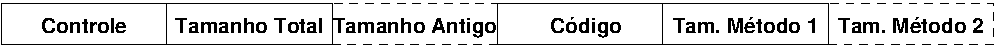
\includegraphics[scale=0.5]{fig/msg_upd} & \\
(c) & \\
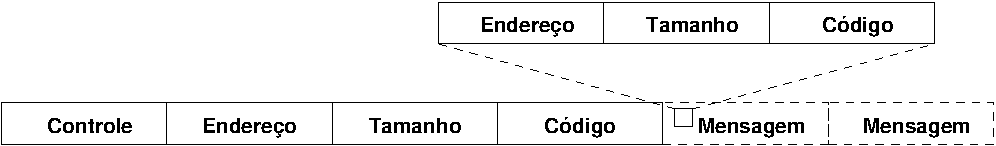
\includegraphics[scale=0.5]{fig/msg_end} & \\
(d) & \\

\includegraphics[scale=0.5]{fig/msg_app} & \\
(e) & \\
\end{tabular}
\caption{Mensagens de reprograma��o do \ETP{}. (a) Adi��o de m�todo (b) Remo��o de m�todo (c) Atualiza��o do componente (d) Atualiza��o de endere�o (e) Atualiza��o da aplica��o (f) Adi��o de atributos.}
\label{fig:etp}
\end{figure}

A mensagem (a) informa uma adi��o de m�todo a um componente. A mensagem (b) informa que um m�todo est� sendo removido de um componente. A mensagem (c) requisita a atualiza��o de todos os m�todos do componente. Para isso, al�m do novo tamanho do c�digo, s�o informados o tamanho antigo, o novo c�digo e o novo tamanho dos m�todos do componente. Todas essas informa��es s�o utilizadas pelo \agent{} para decidir se h� necessidade de alocar novo espa�o de mem�ria ou se o novo c�digo cabe no espa�o antigo. O \ETP{} ainda permite atualizar um endere�o espec�fico (d). V�rias mensagens podem ser concatenadas, e o n�mero de mensagens � controlado pelo campo de controle. A mensagem (e) informa a atualiza��o de uma aplica��o e a mensagem (f) requisita a adi��o de atributos, enviando para o \agent{} o tamanho do objeto que deve ser criado somando os tamanhos dos atributos antigos com os novos. O \agent{} ir� alocar espa�o para o novo objeto contando com os novos atributos, transferir o estado (dados) do objeto antigo para o novo e apagar o objeto antigo. Os atributos s� podem ser acessados atrav�s dos m�todos \componente{set} e \componente{get}, por isso uma mensagem de adi��o de atributos tamb�m deve ser seguida por uma mensagem de adi��o de m�todos.

A estrutura de mensagens criada pelo \ELUS{} permite que um protocolo de dissemina��o de dados seja facilmente integrado ao sistema operacional. O protocolo de dissemina��o deve, portanto, criar mensagens no formato \ETP{} e realizar uma chamada ao \agent{} informando uma atualiza��o. Essa simples estrutura � um diferencial n�o encontrado nos trabalhos relacionados, o que torna o processo de atualiza��o simples e abstrai do desenvolvedor detalhes de como a reprograma��o acontece efetivamente. Al�m disso, n�o � necess�rio reinicializar o sistema, evitando perda de dados, diferentemente dos protocolos de dissemina��o apresentados nos trabalhos relacionados.

A Figura~\ref{fig:sequence_reprog.pdf} apresenta o diagrama de sequ�ncia do processo de atualiza��o, demonstrando como � realizada a integra��o entre o protocolo de dissemina��o de dados e a estrutura do ELUS. O \textsc{Reconfigurator} inicia o protocolo atrav�s da chamada ao m�todo \textit{run}. Este m�todo fica bloqueado at� que uma atualiza��o (nova vers�o) requisitada pelo nodo seja recebida. Ap�s o recebimento dos novos dados, o \textsc{Reconfigurator} cria uma mensagem no formato \ETP{} e passa os dados para o \agent{} atrav�s da chamada ao \textit{trapAgent}. Por fim, o \agent{} realiza a escrita dos dados na mem�ria de c�digo.
 
\fig{sequence_reprog.pdf}{Integra��o do protocolo de dissemina��o com a estrutura do ELUS.}{scale=.7}

\section{Evaluation}
\label{sec:evaluation}
% Memória
% Latência
% Tempo de reconfiguração

%The reprogramming structure formed by \ELUS{} and the dissemination protocol were evaluated in terms of memory consumption, latency of sending data across the network and reconfiguration time.
The infrastructure was evaluated in terms of memory consumption, latency of sending data across the network and reconfiguration time.
%These tests were performed using Mica2\footnote{Sensor node which has an ATMega128 microcontroller, 4KB RAM, 128KB of flash memory, 4KB of EEPROM and radio communication.} nodes.
These tests were performed using Mica2 nodes.
The system was generated with the GNU compiler g++ 4.0.2 and memory consumption measured using the GNU \textit{objdump} 2.16.1 tool.
Latency and reconfiguration times were measured by the timer of the microcontroller.

\subsection{Memory}
Table~\ref{tab:mem} shows the memory consumption of all the framework's elements. For this test, the reconfiguration support was enabled for a component that contains 4 methods. The dissemination protocol occupies 2536 bytes in code area and 21 bytes in the uninitialized data. It is important to notice that a buffer is created dynamically when the new code is received, and its size depends on the size of the update. The \ELUS{} framework consumes 1648 bytes of code, 26 bytes of data and 68 bytes of uninitialized data due to the variables and tables required to store objects and methods.
\begin{table}
\centering
\scriptsize{
%\caption{Consumo de memória da estrutura: \ELUS{} e protocolo de disseminação.}
\caption{Memory consumption of the structure: \ELUS{} and dissemination protocol.}
\begin{tabular}{|c|c|c|c|c|}\hline
\textbf{Structure} & \multicolumn{4}{c|}{\textbf{Section size (bytes)}} \cr
\cline{2-5}
\textbf{Elements} & \textbf{.text} & \textbf{.data} & \textbf{.bss} & \textbf{.bootloader} \cr
\hline
\textbf{Dissemination Protocol} & 2536 & 0 & 21 & 0 \cr\hline
\textbf{\textsc{Reconfigurator}} & 166 & 0 & 4 & 0 \cr\hline
\textbf{AVR Code Manager} & 36 & 0 & 0 & 416 \cr\hline
\textbf{\ELUS{}} & 1648 & 26 & 68 & 0 \cr\hline
\hline
\textbf{Total} & 4386 & 26 & 93 & 416 \cr
\hline
\end{tabular}
\label{tab:mem}
}
\end{table}

Table~\ref{tab:elusMem} shows the memory consumption required by \ELUS{} when a novel component is added to the system. The methods \texttt{Create}, \texttt{Destroy} and \texttt{Update} represent the constructor, destructor and update method for the component, and must always be present. Each component also requires a semaphore to control its exclusive access and prevent an update while the code is running. The minimum consumption to a new component added to the framework is composed of the constructor, destructor, \texttt{Update} method and a method without parameters and without returning value.% , and is 664 bytes of code and 26 bytes of data.
\begin{table}
\centering
\scriptsize{
%\caption{Consumo de memória do \ELUS{} ao habilitar o suporte à reconfiguração em um componente.}
\caption{Memory consumption of \ELUS{} to enable support for a reconfiguration component.}
\begin{tabular}{|c|c|c|}\hline
\textbf{Framework} & \multicolumn{2}{c|}{\textbf{Section Size (bytes)}} \cr
\cline{2-3}
\textbf{Methods} & \textbf{.text} & \textbf{.data} \cr
\hline
Create & 178 & 0 \cr\hline
Destroy & 136 & 0 \cr\hline
Method without parameter & 90 & 0 \cr
and return value & & \cr\hline
Method with parameter & 94 & 0 \cr
and without return value & & \cr\hline
Method without parameter & 104 & 0 \cr
and with return value & & \cr\hline
Method with parameter & 122 & 0 \cr
and return value & & \cr\hline
Update & 260 & 0 \cr\hline
Dispatcher & 0 & 2 X (n. of methods) \cr\hline
Semaphore & 0 & 18 \cr\hline
\hline
\textbf{Minimum size} & 664 & 26 \cr
\hline
\end{tabular}
\label{tab:elusMem}
}
\end{table}
%Equation~\ref{for:size} summarizes the extra cost of memory. The size of a component "C" is the sum of the size of all methods, as shown in Table~\ref{tab:elusMem}, with the size of implementation of component's methods. Also, the size of methods \texttt{Create}, \texttt{Destroy} and \texttt{Update} must be added to this sum. The data size is the sum of component data, values of \texttt{Dispatcher} and \texttt{Semaphore} used by \ELUS{}.
Equation~\ref{for:size} summarizes the extra cost of memory.
\begin{equation}
\label{for:size}
Size_{c} = \sum_{i=1}^n (Method_{i}) + Create + Destroy + Update
\end{equation} 
%The proposed specialization through void pointers showed positive results for memory consumption.
Using the specialization through void pointers it was possible to reduce consumption of approximately 1.2KB (more than 50\%). Currently the minimum size for a new component of the system is 664KB instead of 1.6KB from the previous ELUS implementation \cite{Gracioli:2010}.

\subsection{Latency}
%Foram utilizadas duas topologias para medir a latência do protocolo de disseminação, ilustradas na Figura \ref{fig:topology}: (a) a estação base possui comunicação com todos os nodos, (b) a estação base não possui comunicação com um nodo, que está ao alcance dos outros. Em ambas topologias repetiu-se o processo de disseminação vinte vezes, de forma a atualizar um método de um componente do sistema, propagando 10 bytes de dados (utilizados na atualização do método) e 6 bytes de informações de controle (utilizadas pelo protocolo).
%Figure~\ref{fig:topology} shows the topologies used to measure the latency of the dissemination protocol.
%We used two topologies to measure the latency of the dissemination protocol.
%We used two topologies to measure the latency of the dissemination protocol: (i) the base station can communicate with all nodes, and (ii) there are nodes outside the base station reach.
To measure the latency we used two topologies: (i) the base station can communicate with all nodes, and (ii) there are nodes outside the base station reach.
In both topologies we repeated the dissemination process twenty times, in order to update a method of a system component, propagating 10 bytes of data (used in the update method) and 6 bytes of control information (used by the protocol).

%\begin{figure}
%\centering
%\begin{tabular}{cc}
%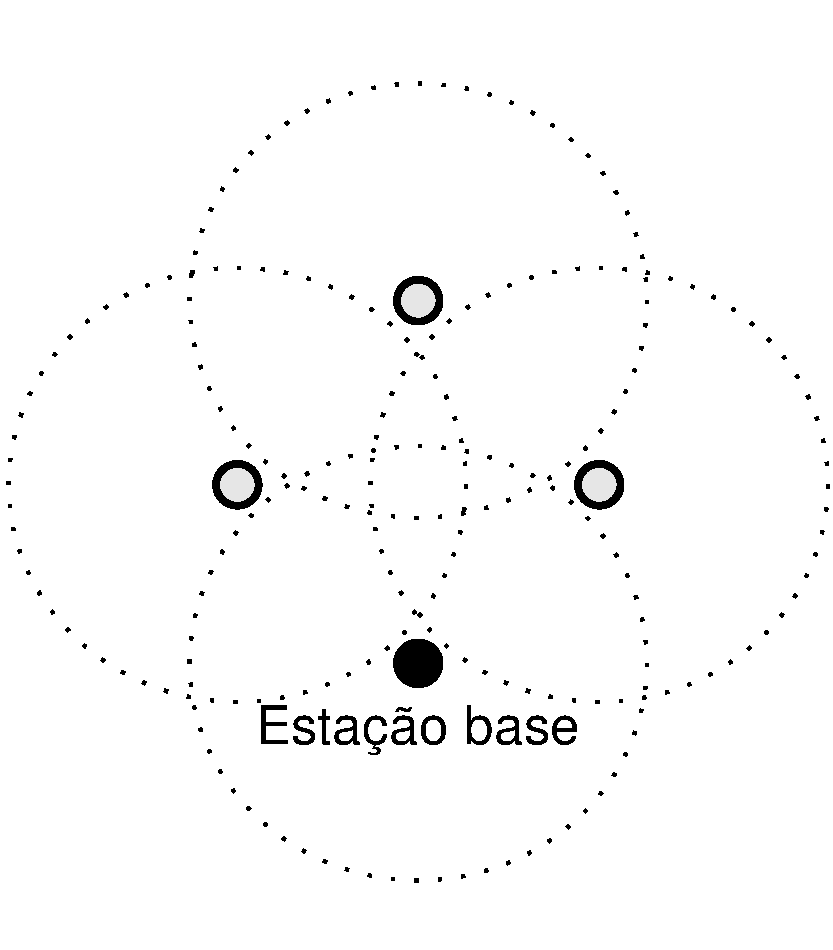
\includegraphics[scale=0.2]{fig/topology1} & 
%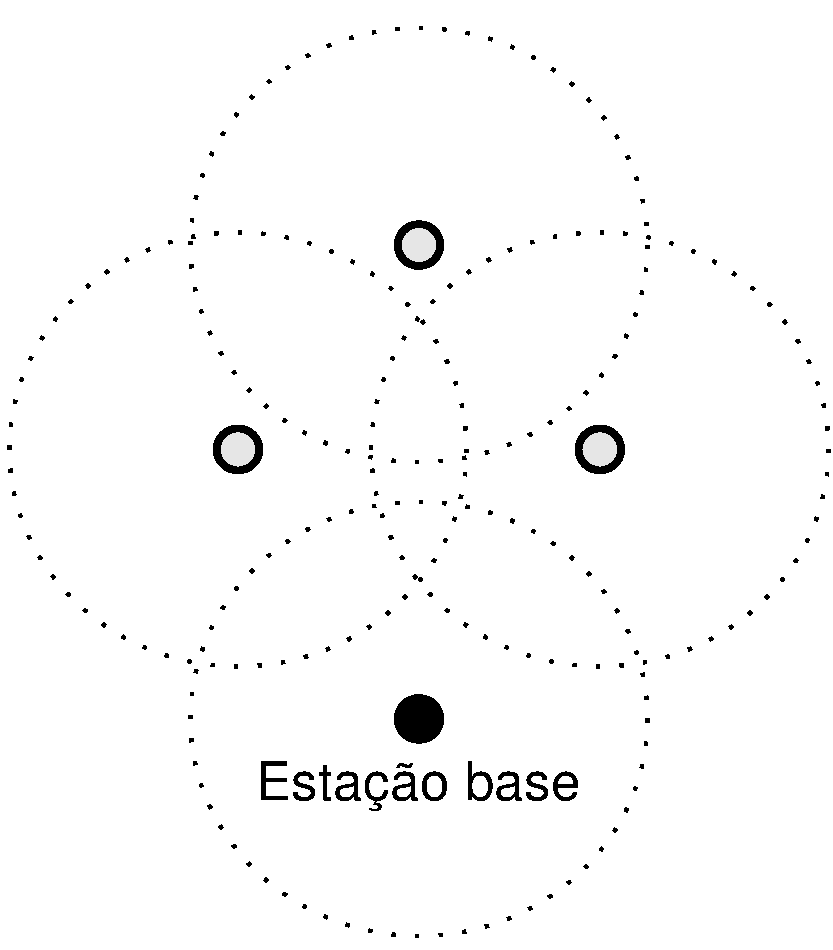
\includegraphics[scale=0.2]{fig/topology2} \\
%(a) & (b)
%\end{tabular}
%\caption{Topologies used to measure the protocol latency. (a) Base station has communication with all nodes (b) Base station does not have communication with all nodes.}
%\label{fig:topology}
%\end{figure}

%A Figura~\ref{fig:latency1} apresenta a média do tempo que a estação base leva para propagar os dados aos nodos a sua volta. Foi observado um desvio padrão de 0,0233 segundos. Este tempo não mudou alterando o número de receptores entre um e três, isto porque pacotes perdidos estão altamente correlacionados, ou seja, vários receptores perdem o mesmo conjunto de pacotes \cite{mnp}.
Figure~\ref{fig:latency1} shows the average time that the base station takes to propagate data to the nodes around it.
We observed a standard deviation of 0.0233 seconds.
This time did not change by changing the number of receivers between one and three.
This happens because loss packet is highly correlated, so multiple receivers lose the same set of packets~\cite{mnp}.

\fig{latency1}{Dissemination and reconfiguration time.}{scale=.57}

%A Figura~\ref{fig:latency2} mostra a média de tempo que os dados levam para serem propagados da estação base para nodos intermediários, e destes para o nodo fora de alcance da estação base (segunda topologia). É possível perceber que o tempo necessário para propagar dados entre nodos normais da rede é aproximadamente quatro vezes maior que o tempo gasto pela estação base, isto se deve ao fato que a estação base não executa a etapa de seleção de emissor, ou seja, não perde tempo divulgando sua versão e recebendo requisições para enfim se tornar um emissor e começar a disseminar os dados. O tempo de disseminação dos nodos intermediários apresentou um desvio padrão de 1,1288 segundos.
Figure~\ref{fig:latency2} shows the average time it takes to propagate the data from the base station to the intermediate nodes, and from these to the node out of range of the base station.
It is possible to notice that the time required to propagate data between normal network nodes is approximately four times greater than the time spent by the base station.
This is due to the fact that the base station does not perform the step of selecting a sender.
This way it wastes no time publishing its version and receiving requests to finally become a sender and begin to disseminate the data.
The time of intermediate nodes had a standard deviation of 1.1288 seconds.
 
\fig{latency2}{Dissemination time.}{scale=.57}

\subsection{Reconfiguration Time}
%Foi considerado como tempo de reconfiguração, o tempo que o nodo leva para atualizar sua memória de programa após ter recebido todos os dados necessários, via o protocolo de disseminação. Na estrutura proposta este tempo engloba: a chamada do \textsc{Reconfigurator}, os métodos \componente{p} e \componente{v} do semáforo, a chamada para o método \componente{Update}, a recuperação dos argumentos passados na mensagem ETP, a recuperação do objeto a ser atualizado em uma tabela hash, descobrir o endereço da \componente{vtable} e a escrita dos dados na flash. A Figura \ref{fig:latency1} mostra a média do tempo de reconfiguração obtido, sendo que o mesmo apresentou um desvio padrão de 0,0103 segundos.
The reconfiguration time encompasses the time a node takes to update its program memory after receiving all the necessary data.
In the proposed structure this time comprises: the call of \textsc{Reconfigurator}, methods \texttt{p} and \texttt{v} of the semaphore, the call to the \texttt{Update}, the recovery of arguments passed on the ETP message, the recovery of the object to be updated in a hash table, find the address of the \texttt{vtable}, and writing data in flash.
Figure~\ref{fig:latency1} shows the average reconfiguration time obtained. 
% It had a standard deviation of 0.0103 seconds. %%%%% isso ta errado

%Uma característica da arquitetura utilizada é que não é possível mudar apenas um byte por vez em sua memória flash. Esta memória só permite a escrita em páginas, cujo tamanho é de 256 bytes, e antes de reescrever uma página é necessário apagar seu conteúdo. Desta forma para atualizarmos uma parte da memória é necessário ler o conteúdo da página e armazená-lo em um buffer temporário, modificar apenas a parte desejada para enfim escrever na flash.
One feature of the Mica2 platform is that it is not possible to change only one byte at a time in its flash memory.
It allows only writing in pages (of 256 bytes), and before rewriting a page it is necessary to delete its contents.
Thus, in order to update a portion of memory, it is necessary to read the page content, store it in a temporary buffer, modify only the desired part of it, and finally write in the flash.


% Summary 

% Contributions: (1) common and simple interface (minor), (2)
% Power-management on embedded systems without using any complex
% high-cost methodology.
In this paper we presented an strategy to enable application-driven
power management in deeply embedded systems. In order to achieve this
goal we allowed application programmers to express when certain
components are not being used. This is expressed through a simple
power management interface which allows power mode switching of system
components, subsystems or the system as a whole, making all
combinations of components operating modes feasible. By using the
hierarchical architecture by which system components are organized in
our system, effective power management was achieved for deeply
embedded systems without the need for costly techniques or strategies,
thus incurring in no unnecessary processing or memory overheads.

A case study using a 8-bit microcontroller to monitor temperature in
an indoor ambient showed that almost 40\% of energy could be saved
when using this strategy. % and with minimal application intervention.

% Problems: concurrence. Describe the Thread problem.

% The paper also listed some identified problems on the path for
% power-aware software and hardware components, discussing and
% explaining how some of these problems have been solved in this work
% and how some of them can be solved, and will be, in future work.

% Even so, it still have its usability.



\bibliographystyle{sbc}
\bibliography{references}

\end{document}
